\chapter{Circuitos de corriente directa}
\section{Resistores en serie y en paralelo}
Cuando se conectan en secuencia varios elementos de circuito, como resistores, baterías y motores con una sola trayectoria de corriente entre los puntos, se dice que están conectados \textbf{en serie}. Se dice que los resistores están conectados \textbf{en paralelo} entre los puntos $a$ y $b$ si cada resistor ofrece una trayectoria alternativa entre los puntos.

Para cualquier combinación de resistores siempre es posible encontrar un resistor \textit{único} que podría remplazar la combinación y dar como resultado la misma corriente y diferencia de potencial totales. La resistencia de este resistor único se llama \textbf{resistencia equivalente} de la combinación.

\subsection{Resistores en serie}
Si los resistores están en \textit{serie}, la corriente $I$ debe ser la misma en todos ellos (la corriente no “se gasta” cuando pasa a través de un circuito). Al aplicar $V=IR$ a cada resistor, se obtiene

\begin{equation*}
V_{ax}=IR_1 \qquad V_{xy}=IR_2 \qquad V_{yb}=IR_3
\end{equation*}

Las diferencias de potencial a través de cada resistor no necesitan ser las mismas (excepto para el caso especial en que las tres resistencias son iguales). La diferencia de potencial $V_{ab}$ a través de toda la combinación es la suma de estas diferencias de potencial individuales:

\begin{equation*}
V_{ab}=V_{ax}+V_{xy}+V_{yb}=I(R_1+R_2+R_3)
\end{equation*}

por lo que 

\begin{equation*}
\frac{V_{ab}}{I}=R_1+R_2+R_3
\end{equation*}

La razón $V_{ab}/I$ es, por definición, la resistencia equivalente $R_{eq}$, por tanto, generalizando, se tiene

\begin{equation}\label{26.1}\marginnote{Resistores en serie}
\boxed{R_{eq}=R_1+R_2+R_3+ \cdots}
\end{equation}

\begin{quote}
La resistencia equivalente de cualquier número de resistores en serie es igual a la suma de sus resistencias indivuduales.
\end{quote}

\subsection{Resistores en paralelo}
Si los resistores están en \textit{paralelo}, la corriente a través de cada resistor no necesita ser la misma, pero la diferencia de potencial entre las terminales de cada resistor debe ser la misma e igual a $V_{ab}$. De $I=V/R$

\begin{equation*}
I_1=\frac{V_{ab}}{R_1} \qquad I_2=\frac{V_{ab}}{R_2} \qquad I_3=\frac{V_{ab}}{R_3}
\end{equation*}

En general, la corriente es diferente a través de cada resistor. Como la carga no se acumula o escapa del punto $a$, la corriente total $I$ debe ser la suma de las tres corrientes en los resistores:

\begin{equation*}
I=I_1+I_2+I_3=V_{ab}\left(\frac{1}{R_1}+\frac{1}{R_2}+\frac{1}{R_3}\right)
\end{equation*}

Generalizando

\begin{equation}\label{26.2}\marginnote{Resistores en paralelo}
\frac{1}{R_{eq}}=\frac{1}{R_1}+\frac{1}{R_2}+\frac{1}{R_3}+\cdots
\end{equation}

\begin{quote}
Para cualquier número de resistores en paralelo, el \textit{recíproco} de la resistencia equivalente es igual a la suma de los recíprocos de sus resistencias individuales.
\end{quote}

\section{Reglas de Kirchhoff}
Una \textbf{unión} en un circuito es el punto en que se unen tres o más conductores. Las uniones también reciben el nombre de \textit{nodos} o \textit{puntos de derivación}. Una \textbf{espira} es cualquier trayectoria cerrada de conducción. Las reglas de Kirchhoff consisten en los dos siguientes enunciados:

\textbf{Regla de Kirchhoff de las uniones:} la suma algebraica de las corrientes en cualquier unión es igual a cero. Es decir,

\begin{equation}\label{26.5}\marginnote{Regla de las uniones, válida en cualquier unión}
\boxed{\sum I=0}
\end{equation}

\textbf{Regla de Kirchhoff de las espiras:} la suma algebraica de las diferencias de potencial en cualquier espira, incluso las asociadas con las fem y las de elementos con resistencia, debe ser igual a cero. Es decir,

\begin{equation}\label{26.6}\marginnote{Regla de las espiras, válida para cualquier espira cerrada}
\boxed{\sum V=0}
\end{equation}

La regla de las uniones se basa en la conservación de la carga eléctrica. La regla de las uniones se basa en la conservación de la carga eléctrica.

\section{Circuitos $R-C$}
\subsection{Carga de un capacitor}

\begin{figure}[h]
\centering
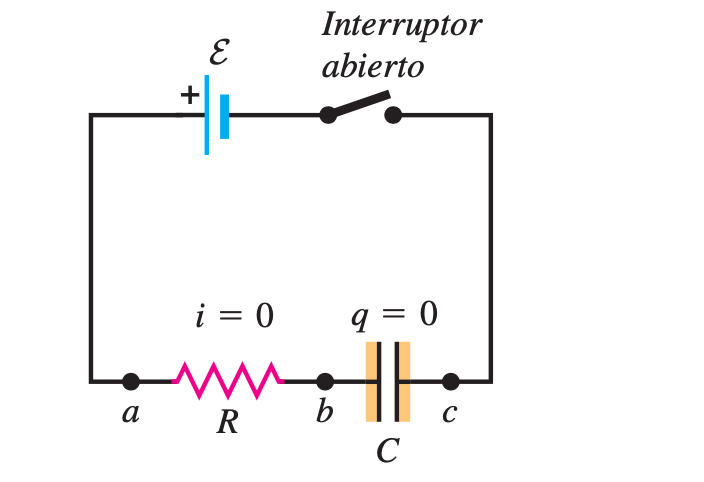
\includegraphics[scale=0.4]{fig/r-c-1}
\caption{Capacitor descargado al inicio. Cuando el interrupor se cierra, a medida que transcurre el tiempo, la carga en el capacitor se incrementa y la corriente disminuye}
\label{fig:r-c-1}
\end{figure}

Un circuito que tiene un resistor y un capacitor conectados en serie, se llama circuito $R-C$ (figura \ref{fig:r-c-1}). Se comienza con el capacitor descargado, después, en cierto momento inicial, $t=0$, se cierra el interruptor, lo que completa el circuito y permite que la corriente alrededor de la espira comience a cargar el capacitor.

Como el capacitor de la figura \ref{fig:r-c-1} al principio está descargado, la diferencia de potencial $v_{bc}$ a través suyo es igual a cero en $t=0$. Después de un periodo largo, el capacitor está cargado por completo, la corriente baja a cero y la diferencia de potencial $v_{ab}$ a través del resistor se vuelve cero. En ese momento aparece la totalidad de la fem $\varepsilon$ de la batería a través del capacitor y $v_{bc}=\varepsilon$. Las diferencias de potencial instantáneas $v_{ab}$ y $v_{bc}$ son

\begin{equation*}
v_{ab}=iR \qquad v_{bc}=\frac{q}{C}
\end{equation*}

Con la regla de Kirchhoff de las espiras, se obtiene

\begin{equation}\label{26.9}
\varepsilon -iR-\frac{q}{C}=0
\end{equation}

Despejando $i$ de la ecuación \ref{26.9}

\begin{equation}\label{26.10}
i=\frac{\varepsilon}{R}-\frac{q}{RC}
\end{equation}

Conforme la carga se incrementa, el término $q/RC$ se hace más grande y la carga del capacitor tiende a su valor final, al que llamaremos $Q_f$. La corriente disminuye y finalmente se vuelve cero. Cuando $i=0$, la ecuación \ref{26.10} da 

\begin{equation}\label{26.11}
\frac{\varepsilon}{R}=\frac{Q_f}{RC} \qquad Q_f=C\varepsilon
\end{equation}

Observe que la carga final $Q_f$ no depende de $R$.

Es posible obtener expresiones generales para la carga $q$ y la corriente $i$ como funciones del tiempo. De ecuación \ref{26.10}
\begin{equation*}
\frac{dq}{dt}=\frac{\varepsilon}{R}-\frac{q}{RC}=-\frac{1}{RC}(1-C\varepsilon)
\end{equation*}
\begin{equation*}
\frac{dq}{q-C\varepsilon}=-\frac{dt}{RC}
\end{equation*}
\begin{equation*}
\int_0^q\frac{dq'}{q'-C\varepsilon}=-\int_0^t\frac{dt'}{RC}
\end{equation*}
\begin{equation*}
\ln\left(\frac{q-C\varepsilon}{-C\varepsilon}\right)=-\frac{t}{RC}
\end{equation*}
\begin{equation*}
\frac{q-C\varepsilon}{-C\varepsilon}=e^{-t/RC}
\end{equation*}

\begin{equation}\label{26.12}\marginnote{Circuito $R-C$, capacitor en carga}
\boxed{q=C\varepsilon \left(1-e^{-t/RC}\right)=Q_f\left(1-e^{-t/RC}\right)}
\end{equation}

Derivando la carga con respecto al tiempo, se tiene

\begin{equation}\label{26.13}\marginnote{Circuito $R-C$, capacitor en carga}
\boxed{i=\frac{dq}{dt}=\frac{\varepsilon}{R}e^{-t/RC}=I_0e^{-t/RC}}
\end{equation}

\subsection{Descarga de un capacitor}

\begin{figure}[h]
\centering
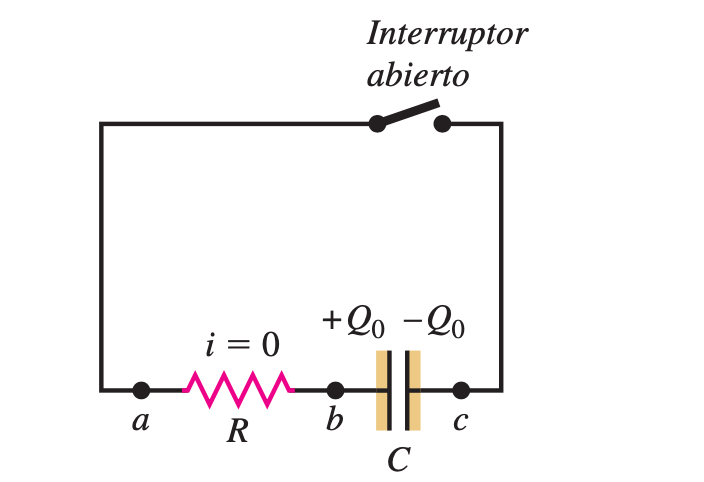
\includegraphics[scale=0.4]{fig/r-c-2}
\caption{Capacitor inicialmente cargado. Cuando se cierra el interruptor, tanto la carga en el capacitor como la corriente disminuyen con el tiempo.}
\label{fig:r-c-2}
\end{figure}

Ahora suponga que después de que el capacitor de la figura \ref{fig:r-c-2} ha adquirido una carga $Q_0$, se retira la batería del circuito $R-C$ y se conectan los puntos $a$ y $c$ a un interruptor abierto. Después se cierra el interruptor y en el mismo instante se reajusta el cronómetro a $t=0$; en ese momento, $q=Q_0$. Luego, el capacitor se descarga a través del resistor y su carga disminuye finalmente a cero. 

Haciendo un cálculo similar al anterior, considerando que en este caso $\varepsilon=0$ en la ecuación de malla, se tiene

\begin{equation}\label{26.16}\marginnote{Circuito $R-C$, capacitor en descarga}
\boxed{q=Q_0e^{-t/RC}}
\end{equation}
Derivando la carga con respecto al tiempo

\begin{equation}\label{26.17}\marginnote{Circuito $R-C$, capacitor en descarga}
\boxed{i=\frac{dq}{dt}=-\frac{Q_0}{RC}=e^{-t/RC}=I_0e^{-t/RC}}
\end{equation}

Mientras el capacitor se carga, la tasa instantánea a la que la batería entrega energía al circuito es $P=\varepsilon i$. La tasa instantánea a la que la energía eléctrica se disipa en el resistor es $i^2R$, y la tasa a que la energía se almacena en el capacitor es $i\, v_{bc}=iq/C$. Al multiplicar la ecuación \ref{26.9} por $i$ se obtiene:

\begin{equation}\label{26.18}
\varepsilon i=i^2R+\frac{iq}{C}
\end{equation}

Esto significa que de la potencia $\varepsilon i$ suministrada por la batería, una parte $(^i2R)$ se disipa en el resistor y otra parte $(iq/C)$ se almacena en el capacitor.

La energía \textit{total} suministrada por la batería durante la carga del capacitor es igual a la fem de la batería $\varepsilon$ multiplicada por el total de la carga $Q_f$, o $\varepsilon Q_f$. La energía total almacenada en el capacitor, según la ecuación \ref{24.9}, es $Q_f \varepsilon/2$. Así, \textit{exactamente} la mitad de la energía suministrada por la batería se almacena en el capacitor, y la otra mitad se disipa en el resistor. Este resultado también se puede verificar en detalle tomando la integral con respecto al tiempo de cada una de las cantidades de potencia en la ecuación \ref{26.18}.




































































